\subsection*{Introduction}

The oceans covering more than 70\% of the Earth's surface are not only
a sink for Carbon, but also a major repository of the global capacity
to store heat from anthropogenic sources. The impact of rising sea
surface temperatures not only impacts marine life, but also human life
deep within terrestrial ecosystems with the increasing mass of heated
air transported from across the oceans over coastal boundaries, to
inland areas. The end result of such transport has led to floods, high
surf, hurricanes and tornados among other extreme events, not just in
coastal zones, but well inland.

\begin{wrapfigure}{r}{0.45\textwidth}
  \centering
  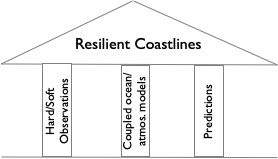
\includegraphics[scale=0.5]{fig/trioka.jpg}
  \caption{Predictive capacity go hand in hand with ocean/land use
    models derived from high resolution sensors from in-situ robotics.}
  \label{fig:tri}
\end{wrapfigure}

To limit loss of life and alleviate human suffering as a result of
such events, technology can and should play a prominent role. Higher
resolution ocean, atmospheric, estuarine and land use models can be
coupled to provide ways to enable 'what-if' analysis for policy makers
and other stakeholders. Increased model skill has resulted in better
predictions, but this is pre-medicated on having higher resolution
data at fine scales. Absent such data, such models cannot be effective
in their forecasting precision. We believe the use of AI-driven
networked mobile robotic platforms carrying a range of payloads in
space, aerial, surface, terrestrial and underwater domains can provide
the necessary capability for precisely such data driven
high-resolution prediction. They can be targeted to be in the 'right
place at the right time' as a result of models being able to bound
their own uncertainty. As a result, the 'three poles' which enable
such a responsive capacity leading to coastal resilience include
observations from hardware robotic platforms, as well as Machine
Learned methods mining troves of remote sensing data all in high
resolution, coupled ocean and atmospheric models which can not only
model the dynamic ocean and its surface, but also interact with
atmospheric phenomenon which provide oceanographic forcing and finally
the predictions for future ocean/atmospheric state which can impact
human habitation inland and on shore (Fig. \ref{fig:tri}).

When these are combined with terrestrial land use, ecological and
hydrological models, a system-of-system then can provide stakeholders,
especially policymakers with a capability for 'what-if' scenario
generation, which in turn can aid in the planning for extreme events
for agencies like FEMA. Such tools can then be used in a number of
ways, foremost being in stress-testing the preparedness of emergency
responders and disaster management agencies, while also providing
strategic advice on asset allocation and placement. Another would be
in using such ensemble modeling for Monte-Carlo type repeat
simulations to come up with the most likely set of scenarios which
could help in building planning resilience. 
